\section{Qt\-File\-Icon\-View Class Reference}
\label{classQtFileIconView}\index{QtFileIconView@{QtFileIconView}}
{\tt \#include $<$qfileiconview.h$>$}

Collaboration diagram for Qt\-File\-Icon\-View:\begin{figure}[H]
\begin{center}
\leavevmode
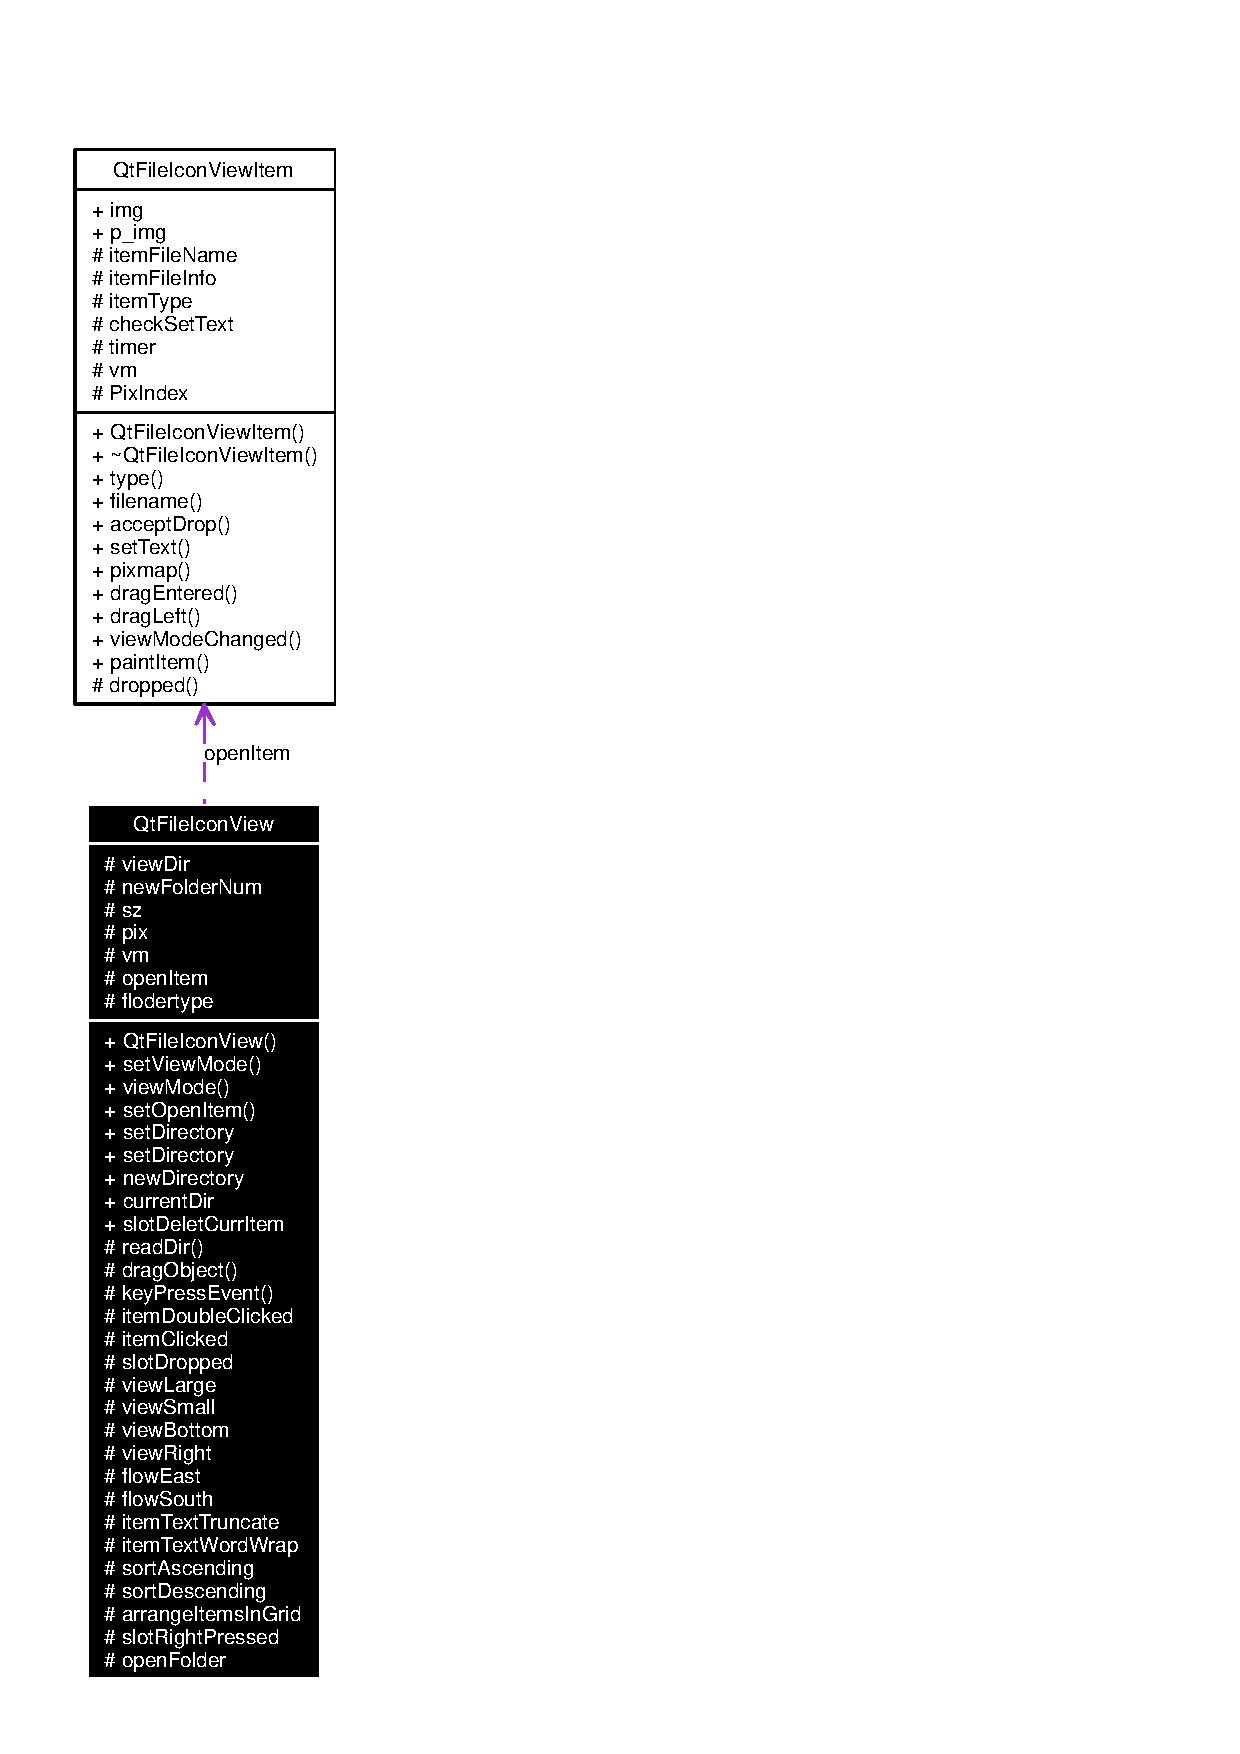
\includegraphics[width=80pt]{classQtFileIconView__coll__graph}
\end{center}
\end{figure}
\subsection*{Public Types}
\begin{CompactItemize}
\item 
enum {\bf View\-Mode} \{ {\bf Large}, 
{\bf Small}
 \}
\end{CompactItemize}
\subsection*{Public Slots}
\begin{CompactItemize}
\item 
void {\bf set\-Directory} (const QString \&dir)
\item 
void {\bf set\-Directory} (const QDir \&dir)
\item 
void {\bf new\-Directory} ()
\item 
QDir {\bf current\-Dir} ()
\item 
void {\bf slot\-Delet\-Curr\-Item} ()
\end{CompactItemize}
\subsection*{Signals}
\begin{CompactItemize}
\item 
void {\bf directory\-Changed} (const QString \&)
\item 
void {\bf start\-Read\-Dir} (int dirs)
\item 
void {\bf read\-Next\-Dir} ()
\item 
void {\bf read\-Dir\-Done} ()
\item 
void {\bf enable\-Up} ()
\item 
void {\bf disable\-Up} ()
\item 
void {\bf enable\-Mkdir} ()
\item 
void {\bf disable\-Mkdir} ()
\item 
void {\bf signal\-Add\-File\-To\-List} (KURL::List list, {\bf HDASS\_\-ACTION\_\-TYPE} act)
\item 
void {\bf signal\-Show\-The\-Detialof\-Image} (KURL url)
\end{CompactItemize}
\subsection*{Public Member Functions}
\begin{CompactItemize}
\item 
{\bf Qt\-File\-Icon\-View} (const QString \&dir, {\bf QWidget} $\ast$parent=0, const char $\ast$name=0,{\bf Floder\-Type} type=Music)
\item 
void {\bf set\-View\-Mode} ({\bf View\-Mode} m)
\item 
{\bf View\-Mode} {\bf view\-Mode} () const 
\item 
void {\bf set\-Open\-Item} ({\bf Qt\-File\-Icon\-View\-Item} $\ast$i)
\end{CompactItemize}
\subsection*{Protected Slots}
\begin{CompactItemize}
\item 
void {\bf item\-Double\-Clicked} (QIcon\-View\-Item $\ast$i)
\item 
void {\bf item\-Clicked} (QIcon\-View\-Item $\ast$i)
\item 
void {\bf slot\-Dropped} (QDrop\-Event $\ast$e, const QValue\-List$<$ QIcon\-Drag\-Item $>$ \&)
\item 
void {\bf view\-Large} ()
\item 
void {\bf view\-Small} ()
\item 
void {\bf view\-Bottom} ()
\item 
void {\bf view\-Right} ()
\item 
void {\bf flow\-East} ()
\item 
void {\bf flow\-South} ()
\item 
void {\bf item\-Text\-Truncate} ()
\item 
void {\bf item\-Text\-Word\-Wrap} ()
\item 
void {\bf sort\-Ascending} ()
\item 
void {\bf sort\-Descending} ()
\item 
void {\bf arrange\-Items\-In\-Grid} ()
\item 
void {\bf slot\-Right\-Pressed} (QIcon\-View\-Item $\ast$item)
\item 
void {\bf open\-Folder} ()
\end{CompactItemize}
\subsection*{Protected Member Functions}
\begin{CompactItemize}
\item 
void {\bf read\-Dir} (const QDir \&dir)
\item 
virtual QDrag\-Object $\ast$ {\bf drag\-Object} ()
\item 
virtual void {\bf key\-Press\-Event} (QKey\-Event $\ast$e)
\end{CompactItemize}
\subsection*{Protected Attributes}
\begin{CompactItemize}
\item 
QDir {\bf view\-Dir}
\item 
int {\bf new\-Folder\-Num}
\item 
QSize {\bf sz}
\item 
QPixmap {\bf pix}
\item 
{\bf View\-Mode} {\bf vm}
\item 
{\bf Qt\-File\-Icon\-View\-Item} $\ast$ {\bf open\-Item}
\item 
{\bf Floder\-Type} {\bf flodertype}
\end{CompactItemize}


\subsection{Member Enumeration Documentation}
\index{QtFileIconView@{Qt\-File\-Icon\-View}!ViewMode@{ViewMode}}
\index{ViewMode@{ViewMode}!QtFileIconView@{Qt\-File\-Icon\-View}}
\subsubsection{\setlength{\rightskip}{0pt plus 5cm}enum {\bf Qt\-File\-Icon\-View::View\-Mode}}\label{classQtFileIconView_QtFileIconVieww2}


\begin{Desc}
\item[Enumeration values: ]\par
\begin{description}
\index{Large@{Large}!QtFileIconView@{QtFileIconView}}\index{QtFileIconView@{QtFileIconView}!Large@{Large}}\item[{\em 
Large\label{classQtFileIconView_QtFileIconVieww2QtFileIconVieww0}
}]\index{Small@{Small}!QtFileIconView@{QtFileIconView}}\index{QtFileIconView@{QtFileIconView}!Small@{Small}}\item[{\em 
Small\label{classQtFileIconView_QtFileIconVieww2QtFileIconVieww1}
}]\end{description}
\end{Desc}



Definition at line 68 of file qfileiconview.h.

Referenced by view\-Mode().



\footnotesize\begin{verbatim}68 { Large, Small };
\end{verbatim}\normalsize 


\subsection{Constructor \& Destructor Documentation}
\index{QtFileIconView@{Qt\-File\-Icon\-View}!QtFileIconView@{QtFileIconView}}
\index{QtFileIconView@{QtFileIconView}!QtFileIconView@{Qt\-File\-Icon\-View}}
\subsubsection{\setlength{\rightskip}{0pt plus 5cm}Qt\-File\-Icon\-View::Qt\-File\-Icon\-View (const QString \& {\em dir}, {\bf QWidget} $\ast$ {\em parent} = 0, const char $\ast$ {\em name} = 0, {\bf Floder\-Type} {\em type} = Music)}\label{classQtFileIconView_QtFileIconViewa0}




Definition at line 272 of file qfileiconview.cpp.

References cleanup(), icon\-File\-Large, item\-Clicked(), item\-Double\-Clicked(), Large, open\-Item, slot\-Dropped(), slot\-Right\-Pressed(), and vm.



\footnotesize\begin{verbatim}273     : QIconView( parent, name ), viewDir( dir ), newFolderNum( 0 ),flodertype(type)
274 {
275    
276         qAddPostRoutine( cleanup );
277         //MP3 File Icon
278         iconFileLarge = new QPixmap( "/root/kde_application/hdass08/skin/mp3icon.png" );
279         vm = Large;
280 
281     setGridX( 75 );
282     setGridY( 75 );
283     setResizeMode( Adjust );
284     setWordWrapIconText( FALSE );
285 
286     connect( this, SIGNAL( doubleClicked( QIconViewItem * ) ),
287              this, SLOT( itemDoubleClicked( QIconViewItem * ) ) );
288     connect( this, SIGNAL( returnPressed( QIconViewItem * ) ),
289              this, SLOT( itemDoubleClicked( QIconViewItem * ) ) );
290     connect( this, SIGNAL( dropped( QDropEvent *, const QValueList<QIconDragItem> & ) ),
291              this, SLOT( slotDropped( QDropEvent *, const QValueList<QIconDragItem> & ) ) );
292     connect( this, SIGNAL( contextMenuRequested( QIconViewItem *, const QPoint & ) ),
293              this, SLOT( slotRightPressed( QIconViewItem * ) ) );
294     connect(this,SIGNAL(clicked( QIconViewItem *)),this,SLOT(itemClicked(QIconViewItem* ))); 
295     setHScrollBarMode( AlwaysOff );
296     setVScrollBarMode( Auto );
297 
298     setAutoArrange( TRUE );
299     setSorting( TRUE );
300     openItem = 0;
301 }
\end{verbatim}\normalsize 


Here is the call graph for this function:\begin{figure}[H]
\begin{center}
\leavevmode

\includegraphics[width=141pt]{classQtFileIconView_QtFileIconViewa0_cgraph}
\end{center}
\end{figure}


\subsection{Member Function Documentation}
\index{QtFileIconView@{Qt\-File\-Icon\-View}!arrangeItemsInGrid@{arrangeItemsInGrid}}
\index{arrangeItemsInGrid@{arrangeItemsInGrid}!QtFileIconView@{Qt\-File\-Icon\-View}}
\subsubsection{\setlength{\rightskip}{0pt plus 5cm}void Qt\-File\-Icon\-View::arrange\-Items\-In\-Grid ()\hspace{0.3cm}{\tt  [inline, protected, slot]}}\label{classQtFileIconView_QtFileIconViewj13}




Definition at line 108 of file qfileiconview.h.

Referenced by set\-View\-Mode(), and slot\-Right\-Pressed().



\footnotesize\begin{verbatim}108                               {
109         QIconView::arrangeItemsInGrid( TRUE );
110     }
\end{verbatim}\normalsize 
\index{QtFileIconView@{Qt\-File\-Icon\-View}!currentDir@{currentDir}}
\index{currentDir@{currentDir}!QtFileIconView@{Qt\-File\-Icon\-View}}
\subsubsection{\setlength{\rightskip}{0pt plus 5cm}QDir Qt\-File\-Icon\-View::current\-Dir ()\hspace{0.3cm}{\tt  [slot]}}\label{classQtFileIconView_QtFileIconViewi3}




Definition at line 349 of file qfileiconview.cpp.

References view\-Dir.



\footnotesize\begin{verbatim}350 {
351     return viewDir;
352 }
\end{verbatim}\normalsize 
\index{QtFileIconView@{Qt\-File\-Icon\-View}!directoryChanged@{directoryChanged}}
\index{directoryChanged@{directoryChanged}!QtFileIconView@{Qt\-File\-Icon\-View}}
\subsubsection{\setlength{\rightskip}{0pt plus 5cm}void Qt\-File\-Icon\-View::directory\-Changed (const QString \&)\hspace{0.3cm}{\tt  [signal]}}\label{classQtFileIconView_QtFileIconViewl0}




Definition at line 247 of file qfileiconview.moc.cc.

Referenced by read\-Dir().



\footnotesize\begin{verbatim}248 {
249     activate_signal( staticMetaObject()->signalOffset() + 0, t0 );
250 }
\end{verbatim}\normalsize 
\index{QtFileIconView@{Qt\-File\-Icon\-View}!disableMkdir@{disableMkdir}}
\index{disableMkdir@{disableMkdir}!QtFileIconView@{Qt\-File\-Icon\-View}}
\subsubsection{\setlength{\rightskip}{0pt plus 5cm}void Qt\-File\-Icon\-View::disable\-Mkdir ()\hspace{0.3cm}{\tt  [signal]}}\label{classQtFileIconView_QtFileIconViewl7}




Definition at line 289 of file qfileiconview.moc.cc.

Referenced by read\-Dir().



\footnotesize\begin{verbatim}290 {
291     activate_signal( staticMetaObject()->signalOffset() + 7 );
292 }
\end{verbatim}\normalsize 
\index{QtFileIconView@{Qt\-File\-Icon\-View}!disableUp@{disableUp}}
\index{disableUp@{disableUp}!QtFileIconView@{Qt\-File\-Icon\-View}}
\subsubsection{\setlength{\rightskip}{0pt plus 5cm}void Qt\-File\-Icon\-View::disable\-Up ()\hspace{0.3cm}{\tt  [signal]}}\label{classQtFileIconView_QtFileIconViewl5}




Definition at line 277 of file qfileiconview.moc.cc.

Referenced by read\-Dir().



\footnotesize\begin{verbatim}278 {
279     activate_signal( staticMetaObject()->signalOffset() + 5 );
280 }
\end{verbatim}\normalsize 
\index{QtFileIconView@{Qt\-File\-Icon\-View}!dragObject@{dragObject}}
\index{dragObject@{dragObject}!QtFileIconView@{Qt\-File\-Icon\-View}}
\subsubsection{\setlength{\rightskip}{0pt plus 5cm}QDrag\-Object $\ast$ Qt\-File\-Icon\-View::drag\-Object ()\hspace{0.3cm}{\tt  [protected, virtual]}}\label{classQtFileIconView_QtFileIconViewb1}




Definition at line 479 of file qfileiconview.cpp.

References Qt\-File\-Icon\-Drag::append(), and Qt\-File\-Icon\-View\-Item::filename().



\footnotesize\begin{verbatim}480 {
481 
482     if ( !currentItem() )
483         return 0;
484 
485     QPoint orig = viewportToContents( viewport()->mapFromGlobal( QCursor::pos() ) );
486     QtFileIconDrag *drag = new QtFileIconDrag( viewport() );
487     drag->setPixmap( *currentItem()->pixmap(),
488                      QPoint( currentItem()->pixmapRect().width() / 2, currentItem()->pixmapRect().height() / 2 ) );
489     for ( QtFileIconViewItem *item = (QtFileIconViewItem*)firstItem(); item;
490           item = (QtFileIconViewItem*)item->nextItem() ) {
491         if ( item->isSelected() ) {
492             QIconDragItem id;
493             id.setData( QCString( item->filename() ) );
494             drag->append( id,
495                           QRect( item->pixmapRect( FALSE ).x() - orig.x(),
496                                  item->pixmapRect( FALSE ).y() - orig.y(),
497                                  item->pixmapRect().width(), item->pixmapRect().height() ),
498                           QRect( item->textRect( FALSE ).x() - orig.x(),
499                                  item->textRect( FALSE ).y() - orig.y(),
500                                  item->textRect().width(), item->textRect().height() ),
501                           QString( item->filename() ) );
502         }
503     }
504     return drag;
505 }
\end{verbatim}\normalsize 


Here is the call graph for this function:\begin{figure}[H]
\begin{center}
\leavevmode
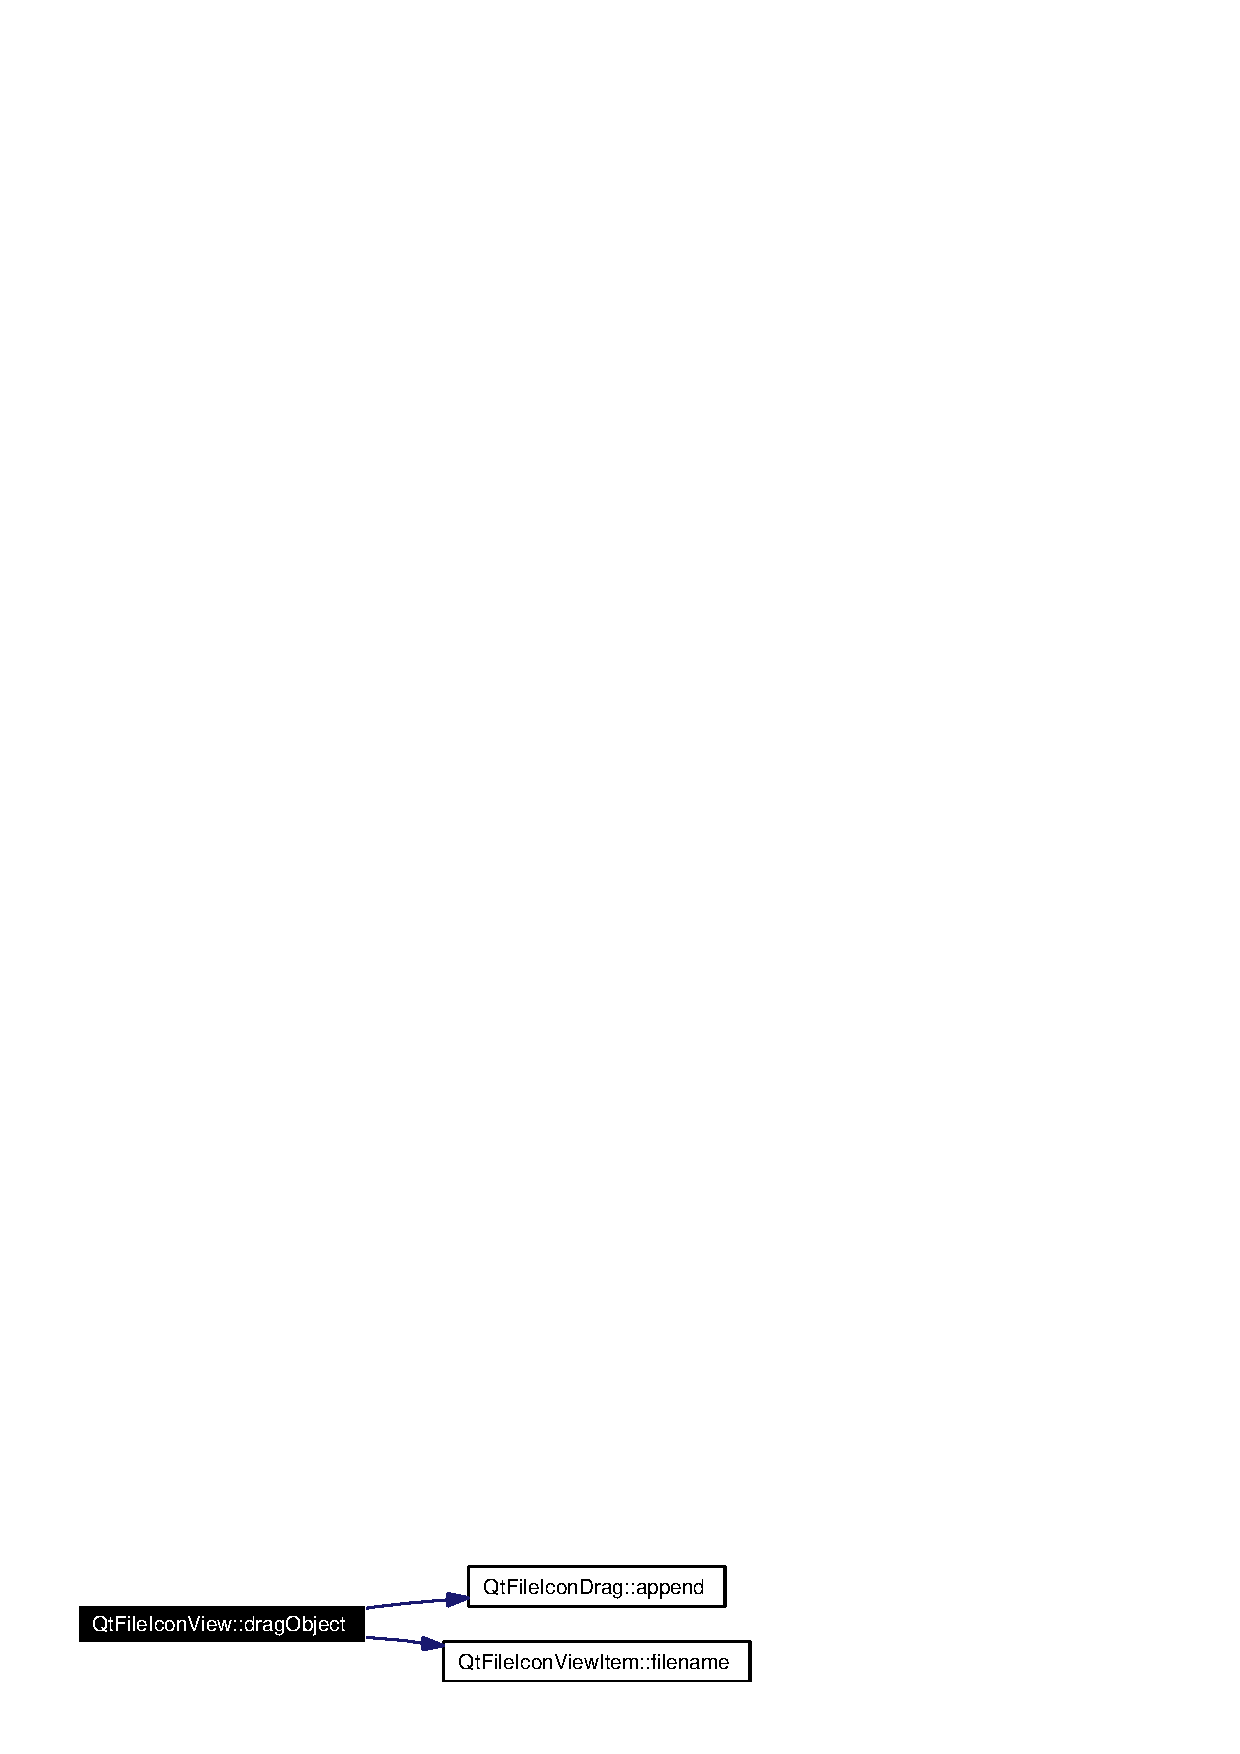
\includegraphics[width=180pt]{classQtFileIconView_QtFileIconViewb1_cgraph}
\end{center}
\end{figure}
\index{QtFileIconView@{Qt\-File\-Icon\-View}!enableMkdir@{enableMkdir}}
\index{enableMkdir@{enableMkdir}!QtFileIconView@{Qt\-File\-Icon\-View}}
\subsubsection{\setlength{\rightskip}{0pt plus 5cm}void Qt\-File\-Icon\-View::enable\-Mkdir ()\hspace{0.3cm}{\tt  [signal]}}\label{classQtFileIconView_QtFileIconViewl6}




Definition at line 283 of file qfileiconview.moc.cc.

Referenced by read\-Dir().



\footnotesize\begin{verbatim}284 {
285     activate_signal( staticMetaObject()->signalOffset() + 6 );
286 }
\end{verbatim}\normalsize 
\index{QtFileIconView@{Qt\-File\-Icon\-View}!enableUp@{enableUp}}
\index{enableUp@{enableUp}!QtFileIconView@{Qt\-File\-Icon\-View}}
\subsubsection{\setlength{\rightskip}{0pt plus 5cm}void Qt\-File\-Icon\-View::enable\-Up ()\hspace{0.3cm}{\tt  [signal]}}\label{classQtFileIconView_QtFileIconViewl4}




Definition at line 271 of file qfileiconview.moc.cc.

Referenced by read\-Dir().



\footnotesize\begin{verbatim}272 {
273     activate_signal( staticMetaObject()->signalOffset() + 4 );
274 }
\end{verbatim}\normalsize 
\index{QtFileIconView@{Qt\-File\-Icon\-View}!flowEast@{flowEast}}
\index{flowEast@{flowEast}!QtFileIconView@{Qt\-File\-Icon\-View}}
\subsubsection{\setlength{\rightskip}{0pt plus 5cm}void Qt\-File\-Icon\-View::flow\-East ()\hspace{0.3cm}{\tt  [protected, slot]}}\label{classQtFileIconView_QtFileIconViewj7}




Definition at line 566 of file qfileiconview.cpp.

Referenced by slot\-Right\-Pressed().



\footnotesize\begin{verbatim}567 {
568     setHScrollBarMode( AlwaysOff );
569     setVScrollBarMode( Auto );
570     setArrangement( LeftToRight );
571 }
\end{verbatim}\normalsize 
\index{QtFileIconView@{Qt\-File\-Icon\-View}!flowSouth@{flowSouth}}
\index{flowSouth@{flowSouth}!QtFileIconView@{Qt\-File\-Icon\-View}}
\subsubsection{\setlength{\rightskip}{0pt plus 5cm}void Qt\-File\-Icon\-View::flow\-South ()\hspace{0.3cm}{\tt  [protected, slot]}}\label{classQtFileIconView_QtFileIconViewj8}




Definition at line 573 of file qfileiconview.cpp.

Referenced by slot\-Right\-Pressed().



\footnotesize\begin{verbatim}574 {
575     setVScrollBarMode( AlwaysOff );
576     setHScrollBarMode( Auto );
577     setArrangement( TopToBottom );
578 }
\end{verbatim}\normalsize 
\index{QtFileIconView@{Qt\-File\-Icon\-View}!itemClicked@{itemClicked}}
\index{itemClicked@{itemClicked}!QtFileIconView@{Qt\-File\-Icon\-View}}
\subsubsection{\setlength{\rightskip}{0pt plus 5cm}void Qt\-File\-Icon\-View::item\-Clicked (QIcon\-View\-Item $\ast$ {\em i})\hspace{0.3cm}{\tt  [protected, slot]}}\label{classQtFileIconView_QtFileIconViewj1}




Definition at line 679 of file qfileiconview.cpp.

Referenced by Qt\-File\-Icon\-View().



\footnotesize\begin{verbatim}680 {
681   QtFileIconViewItem *item = ( QtFileIconViewItem* )i;
682   setCurrentItem(i);
683   //qWarning(item->filename());
684 }\end{verbatim}\normalsize 
\index{QtFileIconView@{Qt\-File\-Icon\-View}!itemDoubleClicked@{itemDoubleClicked}}
\index{itemDoubleClicked@{itemDoubleClicked}!QtFileIconView@{Qt\-File\-Icon\-View}}
\subsubsection{\setlength{\rightskip}{0pt plus 5cm}void Qt\-File\-Icon\-View::item\-Double\-Clicked (QIcon\-View\-Item $\ast$ {\em i})\hspace{0.3cm}{\tt  [protected, slot]}}\label{classQtFileIconView_QtFileIconViewj0}




Definition at line 441 of file qfileiconview.cpp.

References Qt\-File\-Icon\-View\-Item::filename(), mm\_\-append, read\-Dir(), signal\-Add\-File\-To\-List(), signal\-Show\-The\-Detialof\-Image(), Qt\-File\-Icon\-View\-Item::type(), and view\-Dir.

Referenced by Qt\-File\-Icon\-View().



\footnotesize\begin{verbatim}442 {
443     //qWarning("DAVID Test for itemDoubleClicked!!");
444     QtFileIconViewItem *item = ( QtFileIconViewItem* )i;
445     if ( item->type() == QtFileIconViewItem::Dir ) 
446     {
447         viewDir = QDir( item->filename() );
448         readDir( viewDir );
449     } 
450     else if ( item->type() == QtFileIconViewItem::Link && QFileInfo( QFileInfo( item->filename() ).readLink() ).isDir() ) 
451     {
452         viewDir = QDir( QFileInfo( item->filename() ).readLink() );
453         readDir( viewDir );
454     }
455     
456     //DAVID  If double clicked ,then send the file item to the playlist.
457     
458     //DAVID Check that if the file type,u just need to send mp3 file to the playlist.
459     else if(item->type()==QtFileIconViewItem::File)//MP3 file
460     {
461         //DAVID send the file path to the playlist.
462         kdDebug()<<item->filename();
463         KURL url(QString("file:")+item->filename());
464         qWarning(url.fileName());
465         KURL::List list;
466         list<<url;
467         emit signalAddFileToList(list,mm_append);
468     }
469     else if(item->type()==QtFileIconViewItem::Image)//Image file
470     {
471         //DAVID Show the detail of Image
472         kdDebug()<<item->filename();
473         KURL url(QString("file:")+item->filename());
474         emit signalShowTheDetialofImage(url);
475     }
476     
477 }
\end{verbatim}\normalsize 
\index{QtFileIconView@{Qt\-File\-Icon\-View}!itemTextTruncate@{itemTextTruncate}}
\index{itemTextTruncate@{itemTextTruncate}!QtFileIconView@{Qt\-File\-Icon\-View}}
\subsubsection{\setlength{\rightskip}{0pt plus 5cm}void Qt\-File\-Icon\-View::item\-Text\-Truncate ()\hspace{0.3cm}{\tt  [protected, slot]}}\label{classQtFileIconView_QtFileIconViewj9}




Definition at line 590 of file qfileiconview.cpp.

Referenced by slot\-Right\-Pressed().



\footnotesize\begin{verbatim}591 {
592     setWordWrapIconText( FALSE );
593 }
\end{verbatim}\normalsize 
\index{QtFileIconView@{Qt\-File\-Icon\-View}!itemTextWordWrap@{itemTextWordWrap}}
\index{itemTextWordWrap@{itemTextWordWrap}!QtFileIconView@{Qt\-File\-Icon\-View}}
\subsubsection{\setlength{\rightskip}{0pt plus 5cm}void Qt\-File\-Icon\-View::item\-Text\-Word\-Wrap ()\hspace{0.3cm}{\tt  [protected, slot]}}\label{classQtFileIconView_QtFileIconViewj10}




Definition at line 595 of file qfileiconview.cpp.

Referenced by slot\-Right\-Pressed().



\footnotesize\begin{verbatim}596 {
597     setWordWrapIconText( TRUE );
598 }
\end{verbatim}\normalsize 
\index{QtFileIconView@{Qt\-File\-Icon\-View}!keyPressEvent@{keyPressEvent}}
\index{keyPressEvent@{keyPressEvent}!QtFileIconView@{Qt\-File\-Icon\-View}}
\subsubsection{\setlength{\rightskip}{0pt plus 5cm}void Qt\-File\-Icon\-View::key\-Press\-Event (QKey\-Event $\ast$ {\em e})\hspace{0.3cm}{\tt  [protected, virtual]}}\label{classQtFileIconView_QtFileIconViewb2}




Definition at line 507 of file qfileiconview.cpp.

References new\-Directory().



\footnotesize\begin{verbatim}508 {
509     if ( e->key() == Key_N &&
510          ( e->state() & ControlButton ) )
511         newDirectory();
512     else
513         QIconView::keyPressEvent( e );
514 }
\end{verbatim}\normalsize 
\index{QtFileIconView@{Qt\-File\-Icon\-View}!newDirectory@{newDirectory}}
\index{newDirectory@{newDirectory}!QtFileIconView@{Qt\-File\-Icon\-View}}
\subsubsection{\setlength{\rightskip}{0pt plus 5cm}void Qt\-File\-Icon\-View::new\-Directory ()\hspace{0.3cm}{\tt  [slot]}}\label{classQtFileIconView_QtFileIconViewi2}




Definition at line 328 of file qfileiconview.cpp.

References new\-Folder\-Num, and view\-Dir.

Referenced by key\-Press\-Event().



\footnotesize\begin{verbatim}329 {
330     setAutoArrange( FALSE );
331     selectAll( FALSE );
332     if ( viewDir.mkdir( QString( "New Folder %1" ).arg( ++newFolderNum ) ) ) 
333     {                                                                        
334         QFileInfo *fi = new QFileInfo( viewDir, QString( "New Folder %1" ).arg( newFolderNum ) );
335         QtFileIconViewItem *item = new QtFileIconViewItem( this, new QFileInfo( *fi ) ,0);
336         item->setKey( QString( "000000%1" ).arg( fi->fileName() ) );
337         delete fi;
338         repaintContents( contentsX(), contentsY(), contentsWidth(), contentsHeight(), FALSE );
339         ensureItemVisible( item );
340         item->setSelected( TRUE, TRUE );
341         setCurrentItem( item );
342         repaintItem( item );
343         qApp->processEvents();
344         item->rename();
345     }
346     setAutoArrange( TRUE );
347 }
\end{verbatim}\normalsize 
\index{QtFileIconView@{Qt\-File\-Icon\-View}!openFolder@{openFolder}}
\index{openFolder@{openFolder}!QtFileIconView@{Qt\-File\-Icon\-View}}
\subsubsection{\setlength{\rightskip}{0pt plus 5cm}void Qt\-File\-Icon\-View::open\-Folder ()\hspace{0.3cm}{\tt  [protected, slot]}}\label{classQtFileIconView_QtFileIconViewj15}




Definition at line 303 of file qfileiconview.cpp.

References Qt\-File\-Icon\-View\-Item::item\-File\-Name, open\-Item, set\-Directory(), Qt\-File\-Icon\-View\-Item::timer, and Qt\-File\-Icon\-View\-Item::type().



\footnotesize\begin{verbatim}304 {
305     if ( !openItem )
306         return;
307     if ( openItem->type() != QtFileIconViewItem::Dir ||
308          openItem->type() == QtFileIconViewItem::Dir &&
309          !QDir( openItem->itemFileName ).isReadable() )
310         return;
311 
312     openItem->timer.stop();
313     setDirectory( openItem->itemFileName );
314 }
\end{verbatim}\normalsize 
\index{QtFileIconView@{Qt\-File\-Icon\-View}!readDir@{readDir}}
\index{readDir@{readDir}!QtFileIconView@{Qt\-File\-Icon\-View}}
\subsubsection{\setlength{\rightskip}{0pt plus 5cm}void Qt\-File\-Icon\-View::read\-Dir (const QDir \& {\em dir})\hspace{0.3cm}{\tt  [protected]}}\label{classQtFileIconView_QtFileIconViewb0}




Definition at line 376 of file qfileiconview.cpp.

References directory\-Changed(), disable\-Mkdir(), disable\-Up(), enable\-Mkdir(), enable\-Up(), flodertype, is\-Root(), Music, read\-Dir\-Done(), read\-Next\-Dir(), and start\-Read\-Dir().

Referenced by item\-Double\-Clicked(), and set\-Directory().



\footnotesize\begin{verbatim}377 {
378    QDir s=dir;
379    if(flodertype==Image)
380    {
381         s.setNameFilter("*.jpg");
382    }
383    else if(flodertype==Music)
384    {
385         s.setNameFilter("*.mp3");
386    }
387    if ( !dir.isReadable() )
388         return;
389 
390     if ( isRoot( dir.absPath() ) )
391         emit disableUp();
392     else
393         emit enableUp();
394 
395     clear();
396 
397     emit directoryChanged( s.absPath() );
398 
399     const QFileInfoList *filist = s.entryInfoList( QDir::Files );
400 
401     emit startReadDir( filist->count() );
402 
403     int pixindex=0;
404     QFileInfoListIterator it( *filist );
405     QFileInfo *fi;
406     bool allowRename = FALSE, allowRenameSet = FALSE;
407     while ( ( fi = it.current() ) != 0 ) {
408         
409         ++it;
410         if ( fi && fi->fileName() == ".." && ( fi->dirPath() == "/" || fi->dirPath().isEmpty() ) )
411             continue;
412         emit readNextDir();
413         QtFileIconViewItem *item = new QtFileIconViewItem( this, new QFileInfo( *fi ),pixindex );
414         if ( fi->isDir() )
415             item->setKey( QString( "000000%1" ).arg( fi->fileName() ) );
416         else
417             item->setKey( fi->fileName() );
418         if ( !allowRenameSet ) {
419             if ( !QFileInfo( fi->absFilePath() ).isWritable() ||
420                  item->text() == "." || item->text() == ".." )
421                 allowRename = FALSE;
422             else
423                 allowRename = TRUE;
424             if ( item->text() == "." || item->text() == ".." )
425                 allowRenameSet = FALSE;
426             else
427                 allowRenameSet = TRUE;
428         }
429         item->setRenameEnabled( allowRename );
430         ++pixindex;
431     }
432 
433     if ( !QFileInfo( s.absPath() ).isWritable() )
434         emit disableMkdir();
435     else
436         emit enableMkdir();
437 
438     emit readDirDone();
439 }
\end{verbatim}\normalsize 


Here is the call graph for this function:\begin{figure}[H]
\begin{center}
\leavevmode

\includegraphics[width=120pt]{classQtFileIconView_QtFileIconViewb0_cgraph}
\end{center}
\end{figure}
\index{QtFileIconView@{Qt\-File\-Icon\-View}!readDirDone@{readDirDone}}
\index{readDirDone@{readDirDone}!QtFileIconView@{Qt\-File\-Icon\-View}}
\subsubsection{\setlength{\rightskip}{0pt plus 5cm}void Qt\-File\-Icon\-View::read\-Dir\-Done ()\hspace{0.3cm}{\tt  [signal]}}\label{classQtFileIconView_QtFileIconViewl3}




Definition at line 265 of file qfileiconview.moc.cc.

Referenced by read\-Dir().



\footnotesize\begin{verbatim}266 {
267     activate_signal( staticMetaObject()->signalOffset() + 3 );
268 }
\end{verbatim}\normalsize 
\index{QtFileIconView@{Qt\-File\-Icon\-View}!readNextDir@{readNextDir}}
\index{readNextDir@{readNextDir}!QtFileIconView@{Qt\-File\-Icon\-View}}
\subsubsection{\setlength{\rightskip}{0pt plus 5cm}void Qt\-File\-Icon\-View::read\-Next\-Dir ()\hspace{0.3cm}{\tt  [signal]}}\label{classQtFileIconView_QtFileIconViewl2}




Definition at line 259 of file qfileiconview.moc.cc.

Referenced by read\-Dir().



\footnotesize\begin{verbatim}260 {
261     activate_signal( staticMetaObject()->signalOffset() + 2 );
262 }
\end{verbatim}\normalsize 
\index{QtFileIconView@{Qt\-File\-Icon\-View}!setDirectory@{setDirectory}}
\index{setDirectory@{setDirectory}!QtFileIconView@{Qt\-File\-Icon\-View}}
\subsubsection{\setlength{\rightskip}{0pt plus 5cm}void Qt\-File\-Icon\-View::set\-Directory (const QDir \& {\em dir})\hspace{0.3cm}{\tt  [slot]}}\label{classQtFileIconView_QtFileIconViewi1}




Definition at line 322 of file qfileiconview.cpp.

References read\-Dir(), and view\-Dir.



\footnotesize\begin{verbatim}323 {
324     viewDir = dir;
325     readDir( viewDir );
326 }
\end{verbatim}\normalsize 
\index{QtFileIconView@{Qt\-File\-Icon\-View}!setDirectory@{setDirectory}}
\index{setDirectory@{setDirectory}!QtFileIconView@{Qt\-File\-Icon\-View}}
\subsubsection{\setlength{\rightskip}{0pt plus 5cm}void Qt\-File\-Icon\-View::set\-Directory (const QString \& {\em dir})\hspace{0.3cm}{\tt  [slot]}}\label{classQtFileIconView_QtFileIconViewi0}




Definition at line 316 of file qfileiconview.cpp.

References read\-Dir(), and view\-Dir.

Referenced by open\-Folder().



\footnotesize\begin{verbatim}317 {
318     viewDir = QDir( dir );
319     readDir( viewDir );
320 }
\end{verbatim}\normalsize 
\index{QtFileIconView@{Qt\-File\-Icon\-View}!setOpenItem@{setOpenItem}}
\index{setOpenItem@{setOpenItem}!QtFileIconView@{Qt\-File\-Icon\-View}}
\subsubsection{\setlength{\rightskip}{0pt plus 5cm}void Qt\-File\-Icon\-View::set\-Open\-Item ({\bf Qt\-File\-Icon\-View\-Item} $\ast$ {\em i})\hspace{0.3cm}{\tt  [inline]}}\label{classQtFileIconView_QtFileIconViewa3}




Definition at line 72 of file qfileiconview.h.

References open\-Item.



\footnotesize\begin{verbatim}72                                               {
73         openItem = i;
74     }
\end{verbatim}\normalsize 
\index{QtFileIconView@{Qt\-File\-Icon\-View}!setViewMode@{setViewMode}}
\index{setViewMode@{setViewMode}!QtFileIconView@{Qt\-File\-Icon\-View}}
\subsubsection{\setlength{\rightskip}{0pt plus 5cm}void Qt\-File\-Icon\-View::set\-View\-Mode ({\bf View\-Mode} {\em m})}\label{classQtFileIconView_QtFileIconViewa1}




Definition at line 646 of file qfileiconview.cpp.

References arrange\-Items\-In\-Grid(), Qt\-File\-Icon\-View\-Item::view\-Mode\-Changed(), and vm.

Referenced by view\-Large(), and view\-Small().



\footnotesize\begin{verbatim}647 {
648     if ( m == vm )
649         return;
650 
651     vm = m;
652     QtFileIconViewItem *item = (QtFileIconViewItem*)firstItem();
653     for ( ; item; item = (QtFileIconViewItem*)item->nextItem() )
654         item->viewModeChanged( vm );
655 
656     arrangeItemsInGrid();
657 }
\end{verbatim}\normalsize 


Here is the call graph for this function:\begin{figure}[H]
\begin{center}
\leavevmode

\includegraphics[width=208pt]{classQtFileIconView_QtFileIconViewa1_cgraph}
\end{center}
\end{figure}
\index{QtFileIconView@{Qt\-File\-Icon\-View}!signalAddFileToList@{signalAddFileToList}}
\index{signalAddFileToList@{signalAddFileToList}!QtFileIconView@{Qt\-File\-Icon\-View}}
\subsubsection{\setlength{\rightskip}{0pt plus 5cm}void Qt\-File\-Icon\-View::signal\-Add\-File\-To\-List (KURL::List {\em list}, {\bf HDASS\_\-ACTION\_\-TYPE} {\em act})\hspace{0.3cm}{\tt  [signal]}}\label{classQtFileIconView_QtFileIconViewl8}




Definition at line 298 of file qfileiconview.moc.cc.

Referenced by item\-Double\-Clicked().



\footnotesize\begin{verbatim}299 {
300     if ( signalsBlocked() )
301         return;
302     QConnectionList *clist = receivers( staticMetaObject()->signalOffset() + 8 );
303     if ( !clist )
304         return;
305     QUObject o[3];
306     static_QUType_ptr.set(o+1,&t0);
307     static_QUType_ptr.set(o+2,&t1);
308     activate_signal( clist, o );
309 }
\end{verbatim}\normalsize 
\index{QtFileIconView@{Qt\-File\-Icon\-View}!signalShowTheDetialofImage@{signalShowTheDetialofImage}}
\index{signalShowTheDetialofImage@{signalShowTheDetialofImage}!QtFileIconView@{Qt\-File\-Icon\-View}}
\subsubsection{\setlength{\rightskip}{0pt plus 5cm}void Qt\-File\-Icon\-View::signal\-Show\-The\-Detialof\-Image (KURL {\em url})\hspace{0.3cm}{\tt  [signal]}}\label{classQtFileIconView_QtFileIconViewl9}




Definition at line 312 of file qfileiconview.moc.cc.

Referenced by item\-Double\-Clicked().



\footnotesize\begin{verbatim}313 {
314     if ( signalsBlocked() )
315         return;
316     QConnectionList *clist = receivers( staticMetaObject()->signalOffset() + 9 );
317     if ( !clist )
318         return;
319     QUObject o[2];
320     static_QUType_ptr.set(o+1,&t0);
321     activate_signal( clist, o );
322 }
\end{verbatim}\normalsize 
\index{QtFileIconView@{Qt\-File\-Icon\-View}!slotDeletCurrItem@{slotDeletCurrItem}}
\index{slotDeletCurrItem@{slotDeletCurrItem}!QtFileIconView@{Qt\-File\-Icon\-View}}
\subsubsection{\setlength{\rightskip}{0pt plus 5cm}void Qt\-File\-Icon\-View::slot\-Delet\-Curr\-Item ()\hspace{0.3cm}{\tt  [slot]}}\label{classQtFileIconView_QtFileIconViewi4}




Definition at line 658 of file qfileiconview.cpp.

References Qt\-File\-Icon\-View\-Item::filename().

Referenced by mediamanagement::slot\-Delete\-Item().



\footnotesize\begin{verbatim}659 {
660 
661  QtFileIconViewItem *item=( QtFileIconViewItem* )firstItem();
662  while(item)
663  {
664         if(item->isSelected())
665         {
666                 QFile deletefile(item->filename());
667                 deletefile.remove();
668                 QtFileIconViewItem *curitem=item;
669                 item=( QtFileIconViewItem* )item->nextItem();
670                 delete curitem;
671         }
672         else
673         {
674                 item=( QtFileIconViewItem* )item->nextItem();
675         }
676  }
677  sort();
678 }
\end{verbatim}\normalsize 
\index{QtFileIconView@{Qt\-File\-Icon\-View}!slotDropped@{slotDropped}}
\index{slotDropped@{slotDropped}!QtFileIconView@{Qt\-File\-Icon\-View}}
\subsubsection{\setlength{\rightskip}{0pt plus 5cm}void Qt\-File\-Icon\-View::slot\-Dropped (QDrop\-Event $\ast$ {\em e}, const QValue\-List$<$ QIcon\-Drag\-Item $>$ \&)\hspace{0.3cm}{\tt  [protected, slot]}}\label{classQtFileIconView_QtFileIconViewj2}




Definition at line 516 of file qfileiconview.cpp.

References open\-Item, Qt\-File\-Icon\-View\-Item::timer, and view\-Dir.

Referenced by Qt\-File\-Icon\-View().



\footnotesize\begin{verbatim}517 {
518     if ( openItem )
519         openItem->timer.stop();
520     if ( !QUriDrag::canDecode( e ) ) {
521         e->ignore();
522         return;
523     }
524 
525     QStringList lst;
526     QUriDrag::decodeLocalFiles( e, lst );
527 
528     QString str;
529     if ( e->action() == QDropEvent::Copy )
530         str = "Copy\n\n";
531     else
532         str = "Move\n\n";
533     for ( uint i = 0; i < lst.count(); ++i )
534         str += QString( "   %1\n" ).arg( QDir::convertSeparators(lst[i]) );
535     str += QString( "\n"
536         "To\n\n"
537         "       %1" ).arg( viewDir.absPath() );
538 
539     QMessageBox::information( this, e->action() == QDropEvent::Copy ? "Copy" : "Move" , str, "Not Implemented" );
540     if ( e->action() == QDropEvent::Move )
541         QMessageBox::information( this, "Remove" , QDir::convertSeparators(lst.join("\n")), "Not Implemented" );
542     e->acceptAction();
543     openItem = 0;
544 }
\end{verbatim}\normalsize 
\index{QtFileIconView@{Qt\-File\-Icon\-View}!slotRightPressed@{slotRightPressed}}
\index{slotRightPressed@{slotRightPressed}!QtFileIconView@{Qt\-File\-Icon\-View}}
\subsubsection{\setlength{\rightskip}{0pt plus 5cm}void Qt\-File\-Icon\-View::slot\-Right\-Pressed (QIcon\-View\-Item $\ast$ {\em item})\hspace{0.3cm}{\tt  [protected, slot]}}\label{classQtFileIconView_QtFileIconViewj14}




Definition at line 600 of file qfileiconview.cpp.

References arrange\-Items\-In\-Grid(), flow\-East(), flow\-South(), item\-Text\-Truncate(), item\-Text\-Word\-Wrap(), sort\-Ascending(), sort\-Descending(), view\-Bottom(), view\-Large(), view\-Right(), and view\-Small().

Referenced by Qt\-File\-Icon\-View().



\footnotesize\begin{verbatim}601 {
602     if ( !item ) { // right pressed on viewport
603         QPopupMenu menu( this );
604 
605         menu.insertItem( "&Large view", this, SLOT( viewLarge() ) );
606         menu.insertItem( "&Small view", this, SLOT( viewSmall() ) );
607         menu.insertSeparator();
608         menu.insertItem( "Text at the &bottom", this, SLOT( viewBottom() ) );
609         menu.insertItem( "Text at the &right", this, SLOT( viewRight() ) );
610         menu.insertSeparator();
611         menu.insertItem( "Arrange l&eft to right", this, SLOT( flowEast() ) );
612         menu.insertItem( "Arrange t&op to bottom", this, SLOT( flowSouth() ) );
613         menu.insertSeparator();
614         menu.insertItem( "&Truncate item text", this, SLOT( itemTextTruncate() ) );
615         menu.insertItem( "&Wordwrap item text", this, SLOT( itemTextWordWrap() ) );
616         menu.insertSeparator();
617         menu.insertItem( "Arrange items in &grid", this, SLOT( arrangeItemsInGrid() ) );
618         menu.insertSeparator();
619         menu.insertItem( "Sort &ascending", this, SLOT( sortAscending() ) );
620         menu.insertItem( "Sort &descending", this, SLOT( sortDescending() ) );
621 
622         menu.setMouseTracking( TRUE );
623         menu.exec( QCursor::pos() );
624     } else { // on item
625         QPopupMenu menu( this );
626 
627         int RENAME_ITEM = menu.insertItem( "Rename Item" );
628         int REMOVE_ITEM = menu.insertItem( "Remove Item" );
629 
630         menu.setMouseTracking( TRUE );
631         int id = menu.exec( QCursor::pos() );
632 
633         if ( id == -1 )
634             return;
635 
636         if ( id == RENAME_ITEM && item->renameEnabled() ) {
637             item->rename();
638         } else if ( id == REMOVE_ITEM ) {
639             delete item;
640             QMessageBox::information( this, "Not implemented!", "Deleting files not implemented yet,\n"
641                                       "The item has only been removed from the view! " );
642         }
643     }
644 }
\end{verbatim}\normalsize 
\index{QtFileIconView@{Qt\-File\-Icon\-View}!sortAscending@{sortAscending}}
\index{sortAscending@{sortAscending}!QtFileIconView@{Qt\-File\-Icon\-View}}
\subsubsection{\setlength{\rightskip}{0pt plus 5cm}void Qt\-File\-Icon\-View::sort\-Ascending ()\hspace{0.3cm}{\tt  [protected, slot]}}\label{classQtFileIconView_QtFileIconViewj11}




Definition at line 580 of file qfileiconview.cpp.

Referenced by slot\-Right\-Pressed().



\footnotesize\begin{verbatim}581 {
582     sort( TRUE );
583 }
\end{verbatim}\normalsize 
\index{QtFileIconView@{Qt\-File\-Icon\-View}!sortDescending@{sortDescending}}
\index{sortDescending@{sortDescending}!QtFileIconView@{Qt\-File\-Icon\-View}}
\subsubsection{\setlength{\rightskip}{0pt plus 5cm}void Qt\-File\-Icon\-View::sort\-Descending ()\hspace{0.3cm}{\tt  [protected, slot]}}\label{classQtFileIconView_QtFileIconViewj12}




Definition at line 585 of file qfileiconview.cpp.

Referenced by slot\-Right\-Pressed().



\footnotesize\begin{verbatim}586 {
587     sort( FALSE );
588 }
\end{verbatim}\normalsize 
\index{QtFileIconView@{Qt\-File\-Icon\-View}!startReadDir@{startReadDir}}
\index{startReadDir@{startReadDir}!QtFileIconView@{Qt\-File\-Icon\-View}}
\subsubsection{\setlength{\rightskip}{0pt plus 5cm}void Qt\-File\-Icon\-View::start\-Read\-Dir (int {\em dirs})\hspace{0.3cm}{\tt  [signal]}}\label{classQtFileIconView_QtFileIconViewl1}




Definition at line 253 of file qfileiconview.moc.cc.

Referenced by read\-Dir().



\footnotesize\begin{verbatim}254 {
255     activate_signal( staticMetaObject()->signalOffset() + 1, t0 );
256 }
\end{verbatim}\normalsize 
\index{QtFileIconView@{Qt\-File\-Icon\-View}!viewBottom@{viewBottom}}
\index{viewBottom@{viewBottom}!QtFileIconView@{Qt\-File\-Icon\-View}}
\subsubsection{\setlength{\rightskip}{0pt plus 5cm}void Qt\-File\-Icon\-View::view\-Bottom ()\hspace{0.3cm}{\tt  [protected, slot]}}\label{classQtFileIconView_QtFileIconViewj5}




Definition at line 556 of file qfileiconview.cpp.

Referenced by slot\-Right\-Pressed().



\footnotesize\begin{verbatim}557 {
558     setItemTextPos( Bottom );
559 }
\end{verbatim}\normalsize 
\index{QtFileIconView@{Qt\-File\-Icon\-View}!viewLarge@{viewLarge}}
\index{viewLarge@{viewLarge}!QtFileIconView@{Qt\-File\-Icon\-View}}
\subsubsection{\setlength{\rightskip}{0pt plus 5cm}void Qt\-File\-Icon\-View::view\-Large ()\hspace{0.3cm}{\tt  [protected, slot]}}\label{classQtFileIconView_QtFileIconViewj3}




Definition at line 546 of file qfileiconview.cpp.

References Large, and set\-View\-Mode().

Referenced by slot\-Right\-Pressed().



\footnotesize\begin{verbatim}547 {
548     setViewMode( Large );
549 }
\end{verbatim}\normalsize 
\index{QtFileIconView@{Qt\-File\-Icon\-View}!viewMode@{viewMode}}
\index{viewMode@{viewMode}!QtFileIconView@{Qt\-File\-Icon\-View}}
\subsubsection{\setlength{\rightskip}{0pt plus 5cm}{\bf View\-Mode} Qt\-File\-Icon\-View::view\-Mode () const\hspace{0.3cm}{\tt  [inline]}}\label{classQtFileIconView_QtFileIconViewa2}




Definition at line 71 of file qfileiconview.h.

References View\-Mode, and vm.



\footnotesize\begin{verbatim}71 { return vm; }
\end{verbatim}\normalsize 
\index{QtFileIconView@{Qt\-File\-Icon\-View}!viewRight@{viewRight}}
\index{viewRight@{viewRight}!QtFileIconView@{Qt\-File\-Icon\-View}}
\subsubsection{\setlength{\rightskip}{0pt plus 5cm}void Qt\-File\-Icon\-View::view\-Right ()\hspace{0.3cm}{\tt  [protected, slot]}}\label{classQtFileIconView_QtFileIconViewj6}




Definition at line 561 of file qfileiconview.cpp.

Referenced by slot\-Right\-Pressed().



\footnotesize\begin{verbatim}562 {
563     setItemTextPos( Right );
564 }
\end{verbatim}\normalsize 
\index{QtFileIconView@{Qt\-File\-Icon\-View}!viewSmall@{viewSmall}}
\index{viewSmall@{viewSmall}!QtFileIconView@{Qt\-File\-Icon\-View}}
\subsubsection{\setlength{\rightskip}{0pt plus 5cm}void Qt\-File\-Icon\-View::view\-Small ()\hspace{0.3cm}{\tt  [protected, slot]}}\label{classQtFileIconView_QtFileIconViewj4}




Definition at line 551 of file qfileiconview.cpp.

References set\-View\-Mode(), and Small.

Referenced by slot\-Right\-Pressed().



\footnotesize\begin{verbatim}552 {
553     setViewMode( Small );
554 }
\end{verbatim}\normalsize 


\subsection{Member Data Documentation}
\index{QtFileIconView@{Qt\-File\-Icon\-View}!flodertype@{flodertype}}
\index{flodertype@{flodertype}!QtFileIconView@{Qt\-File\-Icon\-View}}
\subsubsection{\setlength{\rightskip}{0pt plus 5cm}{\bf Floder\-Type} {\bf Qt\-File\-Icon\-View::flodertype}\hspace{0.3cm}{\tt  [protected]}}\label{classQtFileIconView_QtFileIconViewp6}




Definition at line 127 of file qfileiconview.h.

Referenced by read\-Dir().\index{QtFileIconView@{Qt\-File\-Icon\-View}!newFolderNum@{newFolderNum}}
\index{newFolderNum@{newFolderNum}!QtFileIconView@{Qt\-File\-Icon\-View}}
\subsubsection{\setlength{\rightskip}{0pt plus 5cm}int {\bf Qt\-File\-Icon\-View::new\-Folder\-Num}\hspace{0.3cm}{\tt  [protected]}}\label{classQtFileIconView_QtFileIconViewp1}




Definition at line 122 of file qfileiconview.h.

Referenced by new\-Directory().\index{QtFileIconView@{Qt\-File\-Icon\-View}!openItem@{openItem}}
\index{openItem@{openItem}!QtFileIconView@{Qt\-File\-Icon\-View}}
\subsubsection{\setlength{\rightskip}{0pt plus 5cm}{\bf Qt\-File\-Icon\-View\-Item}$\ast$ {\bf Qt\-File\-Icon\-View::open\-Item}\hspace{0.3cm}{\tt  [protected]}}\label{classQtFileIconView_QtFileIconViewp5}




Definition at line 126 of file qfileiconview.h.

Referenced by open\-Folder(), Qt\-File\-Icon\-View(), set\-Open\-Item(), and slot\-Dropped().\index{QtFileIconView@{Qt\-File\-Icon\-View}!pix@{pix}}
\index{pix@{pix}!QtFileIconView@{Qt\-File\-Icon\-View}}
\subsubsection{\setlength{\rightskip}{0pt plus 5cm}QPixmap {\bf Qt\-File\-Icon\-View::pix}\hspace{0.3cm}{\tt  [protected]}}\label{classQtFileIconView_QtFileIconViewp3}




Definition at line 124 of file qfileiconview.h.\index{QtFileIconView@{Qt\-File\-Icon\-View}!sz@{sz}}
\index{sz@{sz}!QtFileIconView@{Qt\-File\-Icon\-View}}
\subsubsection{\setlength{\rightskip}{0pt plus 5cm}QSize {\bf Qt\-File\-Icon\-View::sz}\hspace{0.3cm}{\tt  [protected]}}\label{classQtFileIconView_QtFileIconViewp2}




Definition at line 123 of file qfileiconview.h.\index{QtFileIconView@{Qt\-File\-Icon\-View}!viewDir@{viewDir}}
\index{viewDir@{viewDir}!QtFileIconView@{Qt\-File\-Icon\-View}}
\subsubsection{\setlength{\rightskip}{0pt plus 5cm}QDir {\bf Qt\-File\-Icon\-View::view\-Dir}\hspace{0.3cm}{\tt  [protected]}}\label{classQtFileIconView_QtFileIconViewp0}




Definition at line 121 of file qfileiconview.h.

Referenced by current\-Dir(), item\-Double\-Clicked(), new\-Directory(), set\-Directory(), and slot\-Dropped().\index{QtFileIconView@{Qt\-File\-Icon\-View}!vm@{vm}}
\index{vm@{vm}!QtFileIconView@{Qt\-File\-Icon\-View}}
\subsubsection{\setlength{\rightskip}{0pt plus 5cm}{\bf View\-Mode} {\bf Qt\-File\-Icon\-View::vm}\hspace{0.3cm}{\tt  [protected]}}\label{classQtFileIconView_QtFileIconViewp4}




Definition at line 125 of file qfileiconview.h.

Referenced by Qt\-File\-Icon\-View(), set\-View\-Mode(), and view\-Mode().

The documentation for this class was generated from the following files:\begin{CompactItemize}
\item 
{\bf qfileiconview.h}\item 
{\bf qfileiconview.moc.cc}\item 
{\bf qfileiconview.cpp}\end{CompactItemize}
